\documentclass[a4paper,10pt]{article}
\usepackage[T1]{fontenc}
\usepackage[utf8]{inputenc}
\usepackage[english]{babel}
\usepackage{lmodern}
\usepackage[top=1.6cm,bottom=1.8cm,left=1.9cm,right=1.9cm]{geometry}
\usepackage{titlesec,enumitem,xcolor,graphicx,lastpage,fancyhdr}
\usepackage{fontawesome5}
\usepackage[hidelinks]{hyperref}

\hypersetup{colorlinks=true,urlcolor=blue!70!black,linkcolor=blue!70!black}
\pagestyle{fancy}\fancyhf{}\renewcommand{\headrulewidth}{0pt}
\fancyfoot[C]{\small\color{gray}Page \thepage\ of \pageref{LastPage}}
\setlength{\parindent}{0pt}

\titleformat{\section}{\large\bfseries\color{blue!70!black}}{}{0em}{}[\vspace{-0.7em}\rule{\textwidth}{0.5pt}]
\titlespacing{\section}{0pt}{9pt}{5pt}
\setlist[itemize]{leftmargin=1.1em,itemsep=2pt,topsep=2pt,parsep=0pt}
\newcommand{\role}[4]{\vspace{3pt}\noindent\hspace{0.6em}\parbox[t]{0.38\textwidth}{\raggedright\textbf{#1}}\hfill\parbox[t]{0.58\textwidth}{\raggedleft\textit{#2}}\\{\textit{#3}\hfill\textit{#4}}\vspace{1pt}}

\begin{document}
\noindent
\begin{minipage}[t]{0.78\textwidth}
\vspace{0pt}
{\huge\bfseries Prabhavit Gupta}\\[8pt]
{\small \faPhone\ +39-351-610-7807 \quad \faEnvelope\ \href{mailto:prabhavitg@gmail.com}{prabhavitg@gmail.com} \quad \faLinkedin\ \href{https://www.linkedin.com/in/prabhavit/}{Linkedin} \quad \faMapMarker*\ Venice, Italy}
\end{minipage}\hfill
\begin{minipage}[t]{0.18\textwidth}
\vspace{0pt}\raggedleft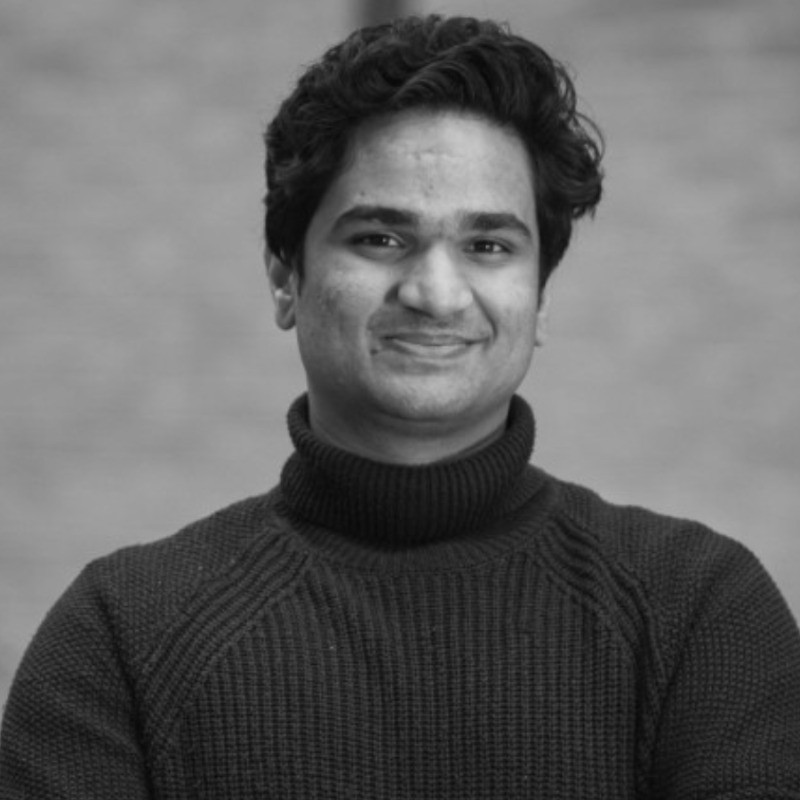
\includegraphics[width=2.3cm,height=2.3cm,keepaspectratio]{photo.jpg}
\end{minipage}

\section{Career Summary}
\begin{itemize}
\item Industrial Automation Software Engineer with a mechanical engineering background and Politecnico di Milano graduate training, specializing in SCADA/HMI systems and industrial data acquisition.
\item Hands-on expertise in Python scripting, SQL relational databases, and connecting supervisory control interfaces with industrial automation hardware.
\item Proven track record in developing real-time operational dashboards, automated monitoring pipelines, and executing structured troubleshooting during testing and commissioning.
\end{itemize}

\section{Technical Skills}
\begin{itemize}
\item \textbf{Industrial Automation \& SCADA} -- SCADA/HMI Systems, Inductive Automation Concepts, Supervisory Dashboards, PLC Interfaces, Data Acquisition
\item \textbf{Programming \& Scripting} -- Python, Jython, SQL, Bash, TypeScript, REST APIs, Git, Linux
\item \textbf{Databases \& Integration} -- PostgreSQL, MySQL, Data Modeling, Real-Time Telemetry, Hardware-Software Integration
\item \textbf{Engineering \& Quality} -- Test Automation, Commissioning Support, Root Cause Analysis, Technical Documentation, System Diagnostics
\end{itemize}

\section{Visa \& Language}
\begin{itemize}
\item \textbf{Language} -- Italian (Conversational / Intermediate), English (Fluent / Professional), Hindi (Native)
\item \textbf{Work Authorization} -- European Long Term Residence Permit - No Sponsorship required.
\end{itemize}

\section{Professional Experience}
\role{\href{https://flowspace.co}{FlowSpace.co}}{Automation Lead Developer (Full time, Freelance)}{London, UK}{Mar 2024 -- Ongoing}
\begin{itemize}
\item \textbf{Industrial Systems \& Monitoring Architecture:}
\begin{itemize}[label=--]
\item Designed supervisory monitoring dashboards and real-time operational telemetry tracking distributed system health.
\item Built automated data ingestion pipelines connecting field endpoints with central PostgreSQL databases via REST APIs.
\item Developed Python scripting modules for automated data processing, anomaly detection, and event alerting.
\item Authored technical architecture specifications, interface definitions, and user manuals for engineering teams.
\end{itemize}
\item \textbf{Operations \& Diagnostics:}
\begin{itemize}[label=--]
\item Maintained 99.9\% system reliability across live operational workflows through proactive error handling and automated recovery.
\item Performed root-cause diagnostic investigations on software exceptions, optimizing payload throughput by 35\%.
\end{itemize}
\item \textit{Tools: Python, SQL, PostgreSQL, Linux, Docker, REST APIs, Git, Jira}
\end{itemize}

\role{Urlink}{Systems Automation Engineer}{Milan, Italy}{Jul 2023 -- Feb 2024}
\begin{itemize}
\item Developed data synchronization services linking connected hardware devices with supervisory relational databases.
\item Implemented automated testing routines and logging frameworks to validate communication integrity across serial and network interfaces.
\item Collaborated with engineering teams during commissioning and deployment phases, verifying operational parameters against technical requirements.
\end{itemize}

\role{UltraStrategy}{Automation Developer}{Remote, Germany}{Sep 2022 -- Jun 2023}
\begin{itemize}
\item Built automated ETL scripts extracting, transforming, and loading operational metrics into analytics databases.
\item Automated diagnostic report generation, reducing manual data auditing time by 40\%.
\end{itemize}

\section{Education}
\role{Politecnico di Milano}{M.Sc. in Management Engineering (Digital Business \& ICT)}{Milan, Italy}{2020 -- 2023}
\role{Thapar Institute of Engineering and Technology}{B.E. in Mechanical Engineering}{Punjab, India}{2014 -- 2018}

\end{document}
